\documentclass[conference]{IEEEtran}

\usepackage{dblfloatfix}
\usepackage{url}
\usepackage{color}
\usepackage{varwidth}
\usepackage[pdftex]{graphicx}
\usepackage{csquotes}
\graphicspath{{./imgs/}{../jpeg/}}
\DeclareGraphicsExtensions{.pdf}
\usepackage{tabularx,booktabs,rotating,multirow}
\usepackage[noadjust]{cite}
\usepackage{caption}
\usepackage[roman]{parnotes}
\usepackage[many]{tcolorbox}
\usepackage[symbol]{footmisc}
\hyphenation{op-tical net-works semi-conduc-tor}
%
% This will go in the next version
%
\makeatletter
\def\parnoteclear{%
    \gdef\PN@text{}%
    \parnotereset
}
\makeatother

\newcolumntype{L}{>{\hsize=.8\hsize\raggedright\arraybackslash}X}
\newcolumntype{R}{>{\raggedleft\arraybackslash}X}
\newcolumntype{C}{>{\centering\arraybackslash}X}
\newcommand\setrow[1]{\gdef\rowmac{#1}#1\ignorespaces}
\newcommand\clearrow{\global\let\rowmac\relax}
\clearrow

%\newcommand\comment[1]{}
%\newcommand{\comment}[1]{{\noindent\bfseries #1\\}}
%\newcommand\todo[1]{{\noindent\color{red}\\\textbf{TODO:~}#1\\}}
\newcommand\todo[1]{}
\newcounter{takeawaycounter}
\setcounter{takeawaycounter}{1}
\renewcommand{\thefootnote}{\fnsymbol{footnote}}

\begin{document}
\title{Software Practitioners' Perspectives on Merge Conflicts and Resolutions}

\author{
\IEEEauthorblockN{Shane McKee\IEEEauthorrefmark{1},
Nicholas Nelson\IEEEauthorrefmark{1},
Anita Sarma,
and Danny Dig}
\IEEEauthorblockA{School of Electrical Engineering and Computer Science\\
Oregon State University,
Corvallis, OR\\ \{mckeesh, nelsonni, anita.sarma, digd\}@oregonstate.edu}}

\maketitle
\thispagestyle{plain}		% REMOVE BEFORE SUBMISSION
\pagestyle{plain}			% REMOVE BEFORE SUBMISSION
\begin{abstract}

When a merge conflict occurs, a developer must investigate the root cause, contributing factors, resources for resolution, plan of action, and any potential after-effects in order to effectively mitigate the conflicting code.
Tool builders and researchers have previously focused on preventing and resolving merge conflicts, but there is little empirical knowledge about how developers rationalize about a conflict while working to resolve it.

In this paper, we present an in-depth empirical study of how developers perceive (1) how to approach merge conflicts, (2) what factors impact the difficulty of a merge conflict resolution, and (3) what toolset changes should be made to improve the resolution process.
To learn more about these perceptions, we interviewed 10 experienced developers, then extended our findings with a survey of 226 developers. We further divided these developers by gender, developer role, experience, source distribution model, and project size.
Our findings suggest that developers have several universal difficulties that cross all demographics, that 
\end{abstract}
\IEEEpeerreviewmaketitle
\section{Introduction}\label{introduction}

\todo{Per Anita's comments, the following prompts needs to be used to rewrite the Introduction section:\\1. What is the problem?\\2. Why is it a problem?\\3. What has been done so far?\\4. What have you done?}

\comment{\textbf{***distributed development process***}}

\comment{\textbf{***Conflicts occur often and cause integration errors****}}
Version control systems like Git offer collaboration via an automated merging process, which enables large-scale distributed development, but they still require manual merging in ambiguous cases called merge conflicts. Sarma et al. \cite{cassandra} show that merge conflicts are as frequent as 19\% of all merges. Resolving merge conflicts can be a costly process that delays projects while developers decide how to approach and resolve the conflict \cite{cassandra}, and poorly-performed merge conflict resolutions frequently cause integration errors \cite{bird-branches-conflict}.

\comment{***current work on proactive detection***}

Several studies have examined models for proactive merge detection and prevention~\cite{Brun2011}\cite{palantir}\cite{Guimaraes}, proposed tools and systems for efficiently avoiding or resolving merge conflicts~\cite{nishimura}\cite{mens2002state}, or discussed advantages of syntax- and semantic-aware merges \cite{danny_refactorings}\cite{hunt2002extensible}. However, at some point in a software projects' development history, there is the chance that a merge conflict will still occur. 

\comment{***we need to know more about conflicts because...***}

Despite the focus in this area, we found no studies that actually talked to developers to understand their perceptions about merge conflicts. Talking directly to developers is crucial to understanding their problems from their perspectives, since some details of merge conflict resolution ---such as cognitive difficulties--- cannot be observed by mining a GitHub repository. For this reason, others such as Gousios et al. \cite{integrator_perspective} have also recognized the importance of directly talking to developers about their problems to better understand integrator difficulties.\\

This paper investigates merge conflicts from the developer standpoint, seeking to understand what developers perceive to be difficult about a merge conflict and the process of resolving it. We then identify target areas for improvement in merge conflict resolution tools. Our research questions reflect these priorities: 

\begin{itemize}
\item\textbf{RQ1:} How do developers approach merge conflicts?\\
\item\textbf{RQ2:} What factors impact the difficulty of a conflict resolution?\\
\item\textbf{RQ3:} Do developer tools meet developer needs for merge conflicts?\\
\end{itemize}

In this study, we interview 10 developers to investigate these research questions, then confirm interview findings in a survey of 226 developers. We provide personal accounts from interviews of experiences in resolving merge conflicts and ranked lists of: the 9 factors that developers use to assess the difficulty of a conflict, the 10 factors that impact developer difficulty while resolving merge conflicts, and 6 tool needs for merge conflict resolution.

When initially assessing the difficulty of a merge conflict, we found developers focus on the code complexity of conflicting lines and their knowledge or expertise in the area of the conflict as the top factors that impact their estimated difficulty, while non-functional changes like whitespace and renaming have little effect on this assessment. 
During the resolution process, we found that developers confirmed code understandability, their knowledge or expertise in the area of the conflict, and the amount of available information about the conflicting code as 3 important factors that impact the difficulty of the resolution.
We also found 6 tool improvements such as better usability and better information filtering, all of which were rated as being moderately 

\section{Methodology}\label{methodology}

\begin{table*}[!t]
\renewcommand{\arraystretch}{1.3}
\caption{Interview Participant Demographics}
\label{interview_demographics}
\centering
\begin{tabularx}{\textwidth}{@{}cl*{2}{C}l*{2}{C}}
\toprule
	\textbf{Partic.} & \textbf{Role} & \textbf{Exp.} & \textbf{Gender} & \textbf{Industry} & \textbf{Project Model} & \textbf{Project Size}\\
\midrule
	P1 & Sr. Software Developer & 18 yrs. & Male & Semiconductor Manuf. & Open-Source & Large\\
	P2 & Software Engineer & 6 yrs. & Male & Semiconductor Manuf. & Open-Source & Large\\
	P3 & Software Engineer & 3 yrs. & Male & Semiconductor Manuf. & Open-Source & Large\\
	P4 & Software Developer & 10 yrs. & Male & Academia & Open-Source & Small\\
	P5 & Infrastructure Engineer & 3 yrs. & Male & Healthcare Software & Closed-Source & Medium\\
	P6 & Software Developer & 5 yrs. & Male & Healthcare Software & Closed-Source & Medium\\
	P7 & Software Engineer & 5 yrs. & Male & Business Software & Open-Source & Medium\\
	P8 & Director & 25 yrs. & Male & Academia & Open-Source & Large\\
	P9 & Collaborator Developer & 8 yrs. & Male & IT Services & Open-Source & Large\\
	P10 & Collaborator Developer & 2 yrs. & Male & Sports \& Wellness Tech. & Open-Source & Small\\
\bottomrule
\end{tabularx}
\end{table*}

Our approach consists of two phases - first an exploratory interview phase, followed by a validation survey. We conducted the interviews with software practitioners who have experience working in team environments. Our goal was to understand the difficulties that developers have when they face merge conflicts and in the conflict resolution process. We followed this with a validation survey to get a wider review of our interview findings.
This two phase approach allowed us to explore the topic of merge conflicts from an individual developer perspective, and to analyze the broader impact of these perspectives on the larger developer population.

\subsection{Interviews}\label{interview_methods}

We conducted semi-structured interviews with software practitioners to discover which factors and concerns they care about when working with merge conflicts.
Interview participants were selected from top contributors to open-source projects and from industry contacts using snowball sampling~\cite{goodman1961snowball}.

Interviews lasted between 30-60 minutes, and were conducted by the first author. 
Interviews were audio-taped and later transcribed for analysis. 
At the beginning of the interview we gave participants a short explanation of the research goals and collected demographics data. 
Participants were then asked about the roles they play in their project, their experience working in team settings,  questions about merge conflicts, the process of conflict resolution, and the difficulties that they faced in conflict resolution. 

The semi-structured interview format allowed participants to provide us with unanticipated information~\cite{seaman2008qualitative}. Further, we allowed open ended discussion about merge conflicts in general at the end of the interview, which allowed participants to share ideas and topics that they found particularly important. 

In total, we interviewed 10 participants (see Table~\ref{interview_demographics}) from six different industries: \textit{Semiconductor Manufacturing} (3 participants), \textit{Healthcare Software} (2), \textit{Academia} (2), \textit{Business Software} (1), \textit{IT Services} (1), and \textit{Sports \& Wellness Technology} (1). The median software development experience was 5 years, and participants worked on a variety of software project sizes; 5 worked primarily on large projects, 3 on medium projects, and 2 on small projects. Participants were offered \$50 for their participation in the interviews.\\

\textit{Analysis:} Interview transcripts were unitized into cards that each contained a single logically consistent statement. This standardized coding scheme was created by the first and second author, and improved to an acceptable point by measure of intercoder  agreement~\cite{unitization}.
Intercoder agreement was determined through \textit{negotiated agreement}, and was reached when no further thematic categories could be created and agreed upon by both coders~\cite{garrison2006revisiting}\cite{ritchie2013qualitative}.
The coding scheme dictated that sentences must be consecutive and topically related to be grouped into a single card. Logically connected statements that were separated by other lines were considered to be separate cards, as a conservative measure to preserve context within each card.

Card sorting is used as a collaborative technique of exploring how people think about a certain topic~\cite{spencer2009card}\cite{card_sort}.
Card sorting allows key concepts and associations to be identified either through open sorting methods (categories are created during the card sorting process) or closed sorting methods (a set of categories is predefined before beginning to card sort).
The card sorting process consists of: deciding upon the topic space, selecting the method (open or closed), gathering the cards, sorting the cards and recording the data, and analyzing the outcomes.
The card sorting process is meant to be collaborative, but argumentative, in order to explore the details of a selected topic.
The process can be repeated several times in order to reach consensus among coders.

The first two authors individually coded emerging themes in the cards and discussed the emerging taxonomies until consensus was reached~\cite{card_sort}.
We performed two iterations of the open card sorting process, and found three themes within our resulting categories: the factors that impact how developers approach merge conflicts (Section~\ref{RQ1}), the difficulties that developers face when resolving conflicts (Section~\ref{RQ2}), and the impact of developer tools on the resolution process (Section~\ref{RQ3}).

%Cards were initially sorted into three categories that corresponded to our research questions before following the typical card sorting workflow [blog cited by Zimmerman in 145 Q's paper]. This workflow requires two people to go through each card and group them by themes. The themes can then be divided into sub-groups or generalized into larger groups.

\subsection{Survey}\label{survey_methods}

\begin{table}[!]
\renewcommand{\arraystretch}{1.3}
\caption{Survey Participant Roles}
\label{survey_roles}
\centering
\begin{tabularx}{0.45\textwidth}{@{}r|*{10}{C}c@{}}
\toprule
\addlinespace[5.4em]
	& \begin{rotate}{45} Soft. Developers \end{rotate} 
	& \begin{rotate}{45} Sys. Architects \end{rotate} 
	& \begin{rotate}{45} DevOps \end{rotate} 
	& \begin{rotate}{45} Project Managers \end{rotate}
	& \begin{rotate}{45} Project Maintainers \end{rotate}
	& \begin{rotate}{45} Sys. Admins \end{rotate}
	& \begin{rotate}{45} Other \end{rotate}\\
\midrule
	Software Developers & 213 & & & & & & \\
	System Architects & 68 & 69 & & & & & \\
	DevOps & 64 & 39 & 68 & & & & \\
	Project Managers & 53 & 32 & 21 & 54 & & & \\
	Project Maintainers & 49 & 27 & 27 & 25 & 50 & & \\
	Systems Administrators & 29 & 22 & 21 & 16 & 15 & 31 & \\
	Other & 9 & 5 & 4 & 4 & 1 & 2 & 11 \\
\bottomrule
\end{tabularx}
\end{table}

We conducted a 50-question survey of software development practitioners in order to examine the themes and categories found in the interviews.
The survey was conducted online and anonymity was guaranteed in order to elicit honest responses from participants.
Questions were developed to confirm, extend, and broaden the results from the interviews.
We wanted to understand which factors impact developers the most when they encounter and resolve merge conflicts.

Survey participants were recruited from contributor lists on open-source repositories on GitHub\footnote{https://github.com/}, advertised on social networking sites (Facebook\footnote{https://www.facebook.com/} and Reddit\footnote{https://www.reddit.com/}), and by directly contacting software developers via email.
We received 226 survey responses, but individual questions have varying response rates and are reported where appropriate in Section~\ref{results}.

The population of 226 survey respondents were overwhelmingly male (91.89\% overall). A majority of respondents considered themselves to be \textit{Software Engineer/Developer} (94.25\% overall, see Table~\ref{survey_roles}). They had a median software development experience of 6-10 years (33.63\% overall), and worked on project sizes ranging from 2-51 developers (the median was 2-5 developers, constituting 49.1\%).

The survey was divided into four categories, with each category containing 5-7 questions (see \cite{companion_site} for questions).
First, we elicited background information about demographics, roles, and experience.
Second, we asked questions related to difficulties that developers experience when encountering merge conflicts.
Third, we asked questions related to conflict resolutions and the factors that affect developers.
Finally we asked questions about the tools and tool features that developers use when working with merge conflicts.
Most questions used a 5-point Likert scale and included an optional open-ended text form to gather additional insights into the questions. 

\textit{Analysis:} We evaluated the distribution of survey answers for each Likert scale question by analyzing across demographic categories. 
We use the mean score for each demographic to determine the positive, negative, or neutral response of the population. 
We considered the third option of the 5-point Likert scale to be neutral, and round scores in the range 2.50 to 3.50 to be equivalent to this neutral response.
\todo{Describe the process of analyzing the survey in light of how we are now coming to our results.}
\section{Results}\label{results}

\subsection{\textbf{RQ1:} How do practitioners approach merge conflicts?}\label{RQ1}
To understand the perspective of practitioners when encountering a merge conflict, we asked interview participants to reflect on situations when they initially face a merge conflict: what kind of information do they seek, how do they approach the resolution of the conflict, and what tools they use. 

We identified nine factors (from card sorting) that practitioners consider when approaching a conflict and attempting to determine its difficulty (see Table~\ref{survey_merge_conflicts}). 
We ask survey participants to rate how each of these nine factors affected their perceptions of difficulty when approaching a merge conflict.
%The survey then asked participants to rate how much each of these 9 factors affected their perceptions of difficulty when approaching a merge conflict. 


We received 162 responses and present the aggregated results in Table~\ref{survey_merge_conflicts}; ranked according to the mean score for each factor.
Here, we discuss in detail the top 4 factors with a mean score greater than $3.00$.
These factors can be grouped into themes of \textit{technical aspects} and \textit{expertise}, and our results are presented according to these groups.

\begin{table*}[!htbp]
\renewcommand{\arraystretch}{1.3}
\caption{Practitioners' Needs for Merge Conflict Resolutions from Survey}
\label{survey_res_diffs}
\centering
\begin{tabularx}{0.87\textwidth}{>{\rowmac}c | >{\rowmac}l | *5{>{\rowmac}c} | *2{>{\rowmac}c}<{\clearrow}}

\toprule
	Need & Description & 1 & 2 & 3 & 4 & 5 & Mean & Median \\
\midrule
	\setrow{\bfseries}N1 & How easy is it to understand the code involved in the merge conflict & 0 & 14 & 25 & 65 & 37 & 3.89 & 4 \\
	\setrow{\bfseries}N2 & Your expertise in the area of code with the merge conflict & 1 & 17 & 38 & 49 & 36 & 3.72 & 4 \\
	\setrow{\bfseries}N3 & The amount of information you have about the conflicting code & 2 & 21 & 38 & 48 & 32 & 3.62 & 4 \\
	\setrow{\bfseries}N4 & How well tools present information in an understandable way & 4 & 24 & 47 & 32 & 34 & 3.48 & 3 \\
	N5 & Changing assumptions within the code & 8 & 27 & 45 & 36 & 25 & 3.30 & 3 \\
	N6 & Complexity of the project structure & 6 & 38 & 39 & 41 & 17 & 3.18 & 3 \\
	N7 & Trustworthiness of tools & 17 & 29 & 39 & 32 & 34 & 3.12 & 3 \\
	N8 & Informativeness of commit messages & 18 & 32 & 30 & 44 & 17 & 3.07 & 3 \\
	N9 & Project culture & 13 & 37 & 43 & 27 & 21 & 3.04 & 3 \\
	N10 & Tool support for examining development history & 16 & 40 & 31 & 32 & 22 & 3.03 & 3 \\
\bottomrule
\end{tabularx}
\vspace*{-0.5\baselineskip}
\end{table*}

\Subsubsection{Technical Aspects}\label{artifact-based-factors}
Two of the top four factors refer to perceptions about the complexity of merge conflicts (F1, F3), with the third factor being \textit{number of conflicting lines} (F4), which can be construed as a specific metric of complexity of the conflict. 
While practitioners mentioned complexity of the lines of code and the file, none mentioned using metrics, such as cyclomatic complexity~\cite{fenton2000quantitative}\cite{mccabe1976complexity} or Function Point Analysis~\cite{garmus2001fpa}\cite{symons1988function}. 
Instead, practitioners made educated guesses on the complexity of the code based on their own experience of either writing the code, or having worked with it. 
Some of the simple to compute metrics, such as \textit{number of conflicting lines of code} (F4), \textit{number of files involved} (F8), \textit{atomicity of changesets} (F6), and \textit{the time} they thought it would take \textit{to resolve the conflict} (F5) were mentioned. 
The only factor where static analysis tools can help was in identifying the \textit{dependencies of the conflicting code} (F7).
This indicates that understanding the complexity of the conflicting code is important, but practitioners do not use the metrics that have been proposed by research. While some of the simple proxies for complexity are used, practitioners primarily rely on their own ``judgement" of the complexity of the conflict.
%Researchers have thus far computed complexity of changes in code using proxies such as lines of code changed and numbers of files changed~\cite{khoshgoftaar1990predicting}.
%Other code-centric metrics such as cyclomatic complexity~\cite{fenton2000quantitative}\cite{mccabe1976complexity} and atomicity changes~\cite{khelladi2016ad} can also be used, but require some amount of computation.
%We found that practitioner's perceptions of complexity are just as important in determining how they approach the resolution of a merge conflict.



This perception of the conflict complexity can affect whether a practitioner resolves the conflict immediately (when small), or whether they should wait to examine the conflict when further resources are available; P8 commented:
\begin{quotation}
\textit{``Small is always easy. A 1-line merge conflict is always easier to resolve than a 400-line merge conflict, and can be done now.''}
\end{quotation}

If a merge conflict is perceived to be large or complex, a practitioner may decide to forgo attempting to resolve it through code manipulation and choose to revert the changes instead~\cite{Guzzi2015}.
This ``nuclear option'' requires practitioners to disrupt the development flow, set aside their current development work, and potentially remove ``good'' code that was not part of the conflict in order to return to a non-conflicting state.
In the interview, P1 describes this process as:
\begin{quotation}
\textit{``If you have many conflicts involved, many commits in the conflict...throw one of the branches away. You cannot combine tens of commits conflicting...it's not sane!''}
\end{quotation}

Further, when integrators are preparing code for production environments they prioritize merge conflicts for code review based upon the perceived difficulty of resolving the affected code.
We find that these decisions rely on humanistic factors as much as they rely on data-driven metrics.
Practitioners may not have the time to compute project-wide complexity metrics, such as those proposed in  literature. Therefore, we need metrics that can be easily calculated by ``lay practitioners" as they face a conflict. 
%are human-aware and take into account the perceived difficulties of merge conflicts.

\Subsubsection{Expertise}\label{knowledge-based-factors}
Our findings show that expertise in the area of conflicting code is one of the top factors in determining the difficulty of a merge conflict (F2). This reiterates the fact that practitioners rely on their own knowledge about the conflicting code base when approaching a conflict. 

Our results indicate that when practitioners feel they don't have the expertise in the conflicting code base, they consider the conflict difficult to merge and seek out more information or assistance from others. 
P5 illustrated this need for expertise when describing his workflow: 
\begin{quotation}
	\textit{``A lot of what I work on is in my own little area...I know what to do\textellipsis But in [unfamiliar part of code], then I'll get someone else to resolve the merge conflict for me. It's someone else's code, and I don't want to screw it up.''}
\end{quotation}



%The importance of the knowledge-based factor indicates that practitioners attribute value to information; the greater knowledge in the conflicting code, the more likely it can be resolved correctly.
%When information is not available, practitioners seek others with expertise to fill this information gap.

%When attempting to resolve a conflict alone, practitioners working in unfamiliar code often feel uncomfortable making decisions during a merge due to lack of familiarity with the code or impacts related to the code change~\cite{CostaSarma}. 
%Situations such as these raise questions relating to which person is best suited to resolve the conflict without introducing a new bug or unintentionally changing code behavior. 

Our findings confirm the need for tools that identify appropriate experts~\cite{CostaSarma} and encourage further research into selection of knowledgeable practitioners for merge conflict resolution.


%We find that expertise, as well as awareness of specific expert knowledge among teams, is an important factor in determining the difficulty of a merge conflict.
%The ability to know who to contact in order to resolve a merge conflict partially explains the drive towards specific integrator and release engineer roles increasing appearing in many software development projects~\cite{adams_release_eng}.

%The results of our survey indicate that \textit{complexity of conflicting lines of code} and \textit{knowledge/expertise in the area of conflicting code} are factors that practitioners find have a direct effect on the perceived difficulty of a merge conflict.
%Although we found consensus across all demographics, the experience level of respondents had an affect on the degree to which they responded affirmatively for these factors (see Table~\ref{survey_merge_conflicts}).
%
%Practitioners with 1-5 years and 6-10 years of experience were only nominally in agreement that merge conflict difficulty is affected by \textit{complexity of conflicting lines of code} (mean: 3.31 and mean: 3.37 respectively) and \textit{knowledge/expertise in the area of conflicting code} (mean: 3.21 and mean: 3.42 respectively).
%As practitioner experiences increases, the level of agreement increases on both of these factors, with practitioners indicating 26+ years experience having the highest consensus (mean: 4.06, std. deviation: 0.77). 
%
%Larger, more complex projects typically require that developers have more experience and a higher degree of knowledge about the systems used in the project.
%As the size of a software project increases, so does the complexity of the underlying code~\cite{banker1993software}\cite{curtis1979third}.
%Therefore, more experienced practitioners are likely to have a broader range of understanding about both \textit{complexity of conflicting lines of code} and \textit{knowledge/expertise in the area of conflicting code} and their affects on merge conflict difficulty.
%
%\begin{figure}[!t]
%\centering
%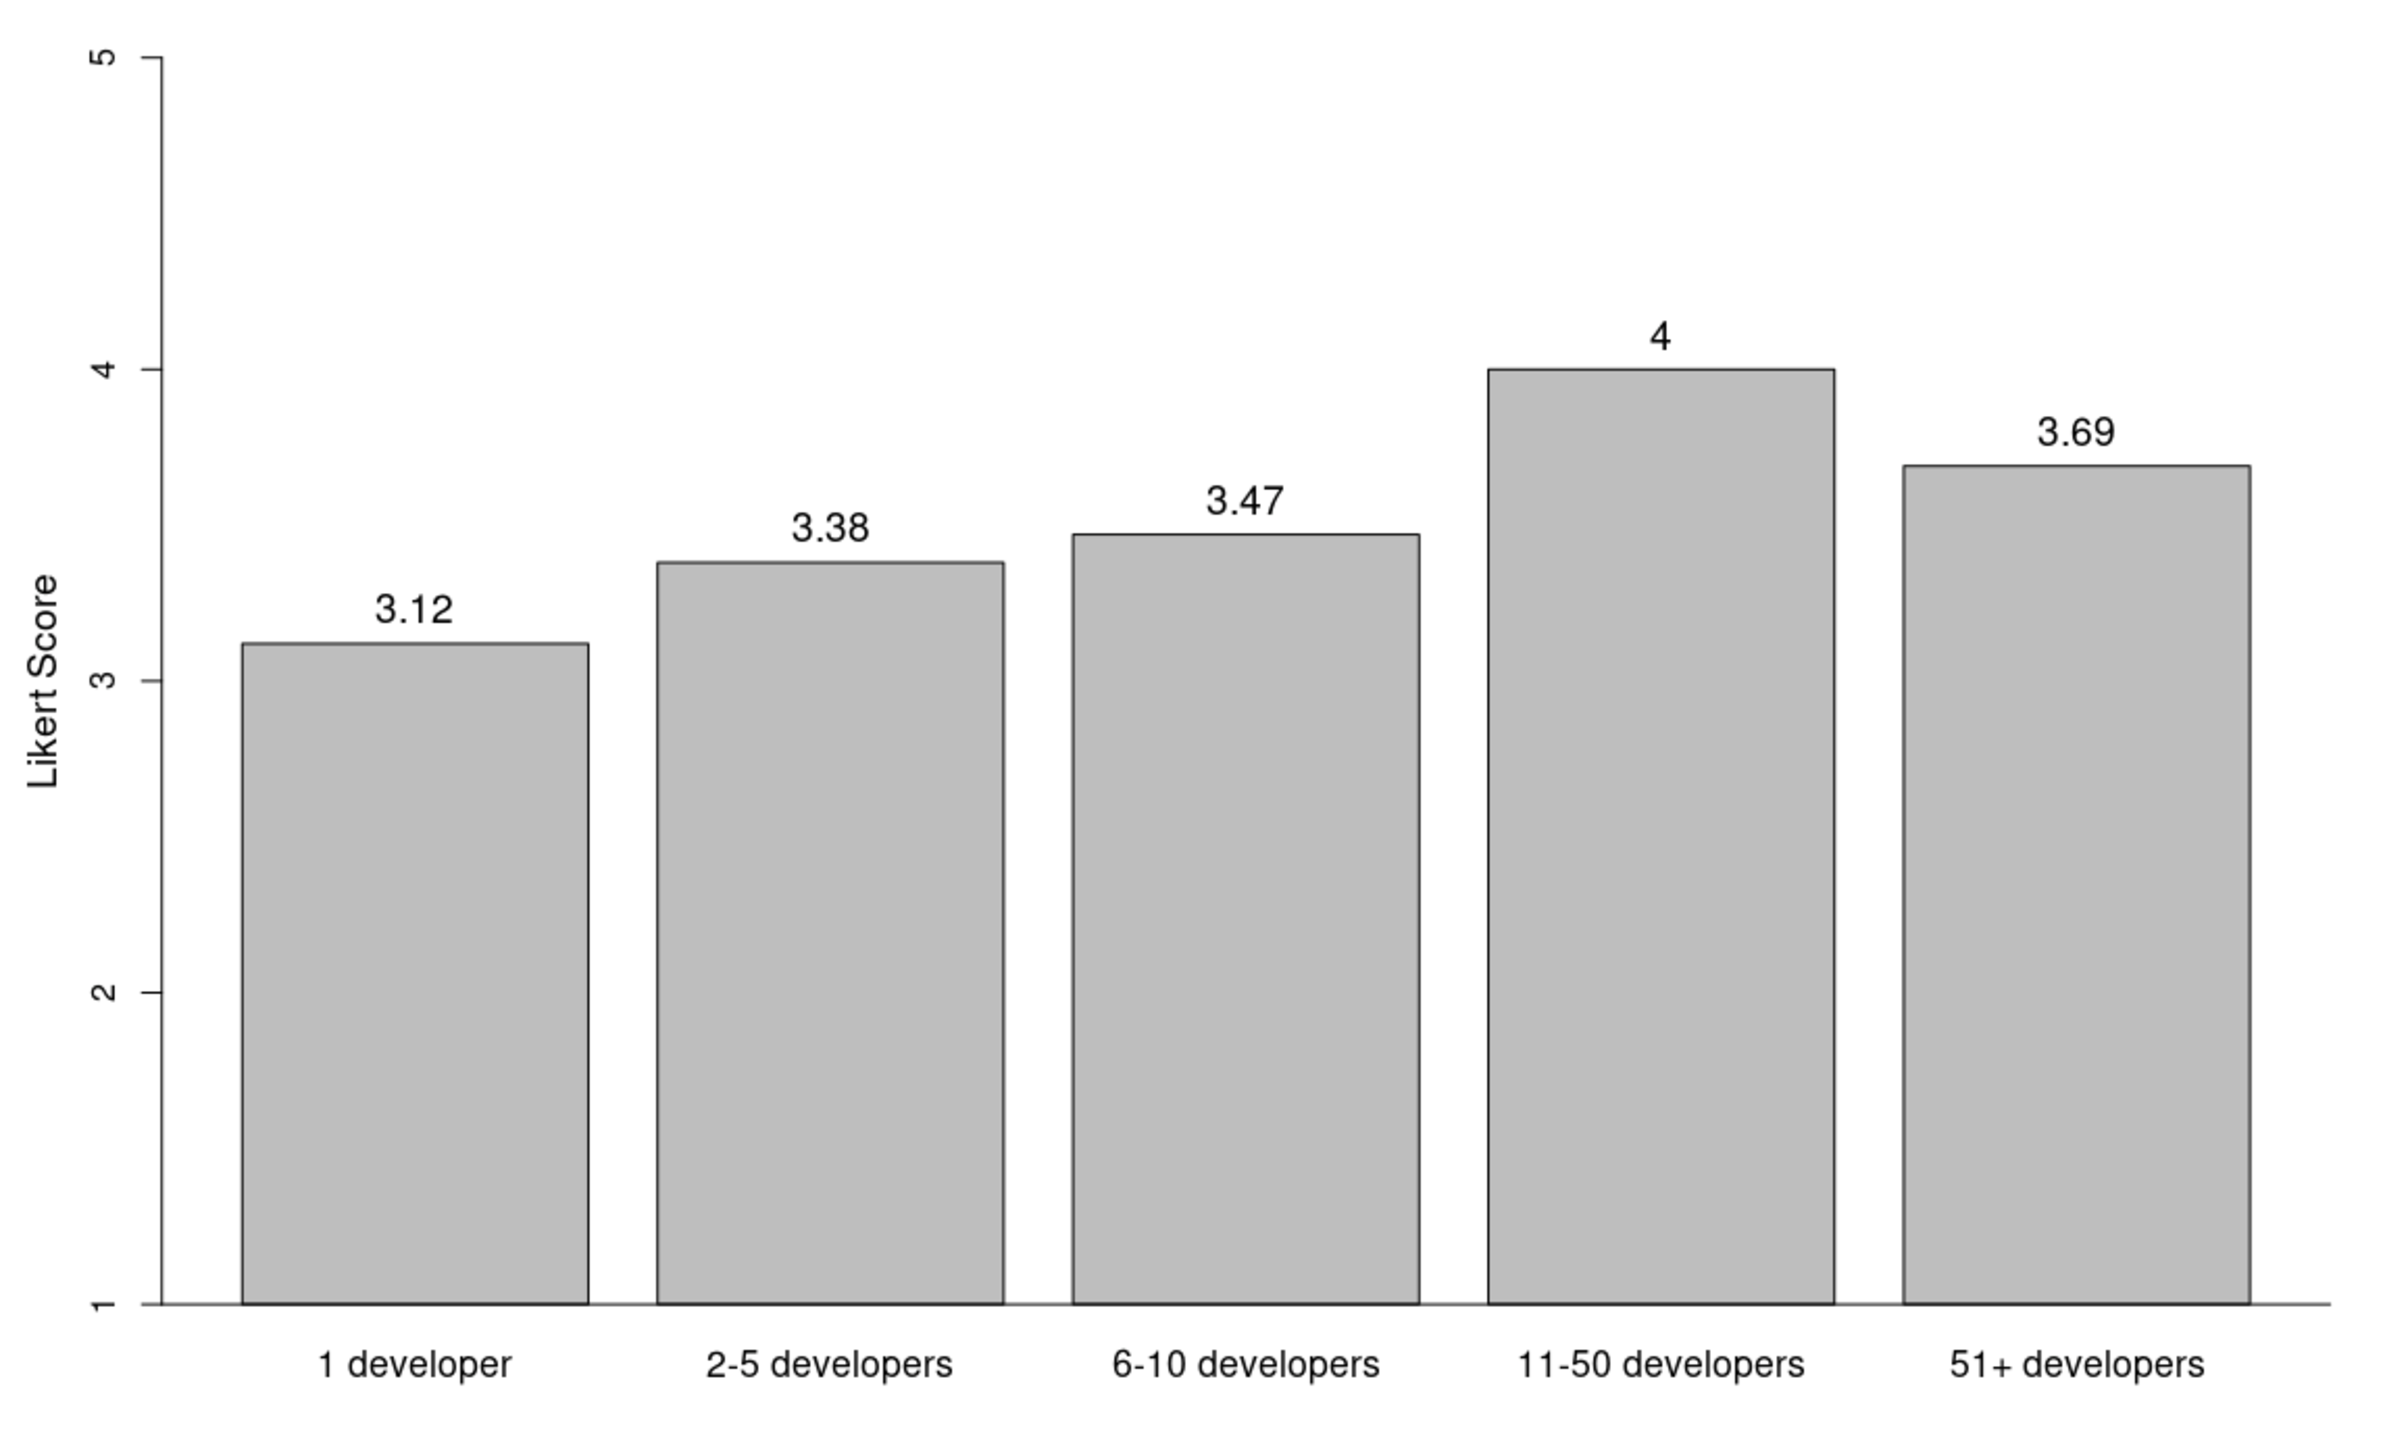
\includegraphics[width=3.4in]{MeanProjectSize.pdf}
%\caption{Mean Likert Score by Project Size for \textit{knowledge/expertise in the area of conflicting code} category of factors that effect the perceived difficulty of merge conflicts.}
%\label{mean_likert_project_size}
%\end{figure}
%
%When analyzing by the size of project that practitioners normally work on, we found that \textit{knowledge/expertise in the area of conflicting code} was increasingly viewed as having an effect on merge conflict difficult as the practitioners' project size increased (see Figure~\ref{mean_likert_project_size}).
%The practitioners that usually work in project sizes of \textit{1 developer}, \textit{2-5 developers}, and \textit{6-10 developers} had relatively neutral responses regarding the effects of \textit{knowledge/expertise in the area of conflicting code} (mean: 3.12, mean: 3.38, and mean: 3.47 respectively).
%However, practitioners that usually work in project sizes of \textit{11-50 developers} and \textit{51+ developers} more positively indicated that \textit{knowledge/expertise in the area of conflicting code} has an effect on the difficulty of merge conflicts (mean: 4.00 and mean: 3.69 respectively).
%
%We also found that practitioners agree that \textit{non-functional changes (whitespace, renaming, etc.)} (mean: 2.16, std. deviation: 1.03) has no effect on the perceived difficulty of a merge conflict.
%Non-functional changes are textual conflicts that can be resolved without consideration of dependencies, performance, or scope.
%Practitioners have less to reason about when resolving merge conflicts that involve only textual conflicts, and therefore are unlikely to perceive \textit{non-functional changes} as affecting the difficulty of merge conflicts.

%Intuitively, we would assume that an increased perception of \textit{knowledge/expertise in the area of conflicting code} as difficulty factor would correlate with a decreased perception of \textit{complexity of conflicting lines of code} as a difficulty factor of merge conflicts.
%This relationship would indicate that a developer's expertise allows them to rationalize about merge conflicts with higher complexity, since they have a higher degree of past knowledge in that area of conflict.
%However, we find a statistical significant correlation between \textit{complexity of conflicting lines of code} and \textit{knowledge/expertise in the area of conflicting code} (Pearson's correlation coefficient: 0.2766, p-value: 0.0003664, 95\% confidence interval: 0.1279 0.4132).
%This suggests that ...

%%%%%%%%%%%%%%%%%%%%%%%%%%%%%%%%%%%%%%%%%%%%%%%%%%%%%%%%%%%%%%%%%

%\subsubsection{Interviews}
%%The interview results suggest that developers approach merge conflicts...
%
%\subsubsection{Survey}
%Our survey suggests that regardless of gender, developer role, experience level, project size, and source distribution model, software practitioners say that the following factors affect the difficulty of a merge conflict most: 
%\begin{itemize}
%\item \textit{Complexity of conflicting lines of code}
%\item \textit{Your knowledge/expertise in area of conflicting code}
%\end{itemize}
%
%Similarly, software practitioners across every measured demographic perceived the following factors to be less important when deciding the difficulty of a merge conflict:
%\begin{itemize}
%\item \textit{Non-functional changes (whitespace, renaming, etc)}
%\item \textit{Number of files in the conflict}
%\end{itemize}
%
%While survey participants did not agree that non-functional changes strongly factor into the difficulty of a merge conflict, it is still worth noting that several interview participants named non-functional changes, such as large refactor or reformatting changes, as a cause for merge conflicts. This suggests that non-functional changes may increase the likelihood of a merge conflict happening, but they do not contribute to the conflict's difficulty.
%
%However, some demographics do view certain difficulties. For instance, open-source developers think that \textit{Atomicity of change sets in the conflict} impacts the difficulty, while closed-source developers and people who split their time evenly think that atomic change sets have no effect on the difficulty. This may be explained by the findings in Rigby et al\cite{OSS_smaller_commits}, which shows that open-source projects tend to review smaller changes than closed-source projects because "The small size lets reviewers focus on the entire change, and the incrementality reduces reviewers’ preparation time and lets them maintain an overall picture of how the change fits into the system." It is possible that our result reflects this difference of culture.
%
%We also found that Project Maintainers say that \textit{Time to resolve a conflict} has an effect, while no other role agrees. This suggests that those in a maintainer role may be more subject to time-related constraints such as maintenance or release schedules. 
%
%\comment{Project Managers say no effect because they focus on project schedules, not conflict resolutions, i.e. they are higher level/abstraction?}
%
%\todo{might be previous work}
%Support and infrastructure roles (System Engineer, Sys Admin, System Architect, DevOps) emphasized that \textit{Dependencies of conflicting code on other components} have more of an effect than other roles did. This might be due to infrastructure systems being maintained in a live environment, or systems that are currently in production use and at risk of real-time dependency failures. 
%
%Developers on projects of size 1 say that \textit{Dependencies of conflicting code on other components}. Because no other project sizes agree with this idea, we hypothesize that this could be due to their high dependence on external code because of the software production limitations of a 1-developer team.
%
%We also found that the group of developers with 21-25 years of experience frequently contradicted general consensus, but it seems more likely that these differences were simply due to the group's small sample size (4).

%We asked participants how much they trust their merging, history exploration, and/or conflict resolution tools, and 57.9\% of participants reported that they trusted these tools either \textit{A Lot} or \textit{Completely}. While this is a majority of developers, this still leaves a significant number of people (42.1\%) who trust their tools \textit{A moderate amount} or \textit{A little}. Though we had the option for \textit{Not at all}, no participants selected this option, presumably because users stop using tools that they do not trust at all. While we found no previous work discussing the threshold for how much users must trust tools for a good tool experience, we postulate that users who cannot trust their tools \textit{A Lot} or \textit{Completely} will avoid relying on such tools too much.
\subsection{\textbf{RQ2:} What unmet needs impact the difficulty of a conflict resolution?}\label{RQ2}

\todo{Story: Everything was important, commit messages have a research bias, Archeology catapults us into RQ3 with motivations}
The perception of merge conflict difficulty and the actual hurdles of resolving them are distinct, and at times separated by a gap in knowledge or awareness that prevent practitioners from accurately gauging the difficulty of resolving merge conflicts.
We asked interview participants a series of open-ended questions regarding unmet needs, the impact of unmet needs on understandability, and their impact on resolving merge conflicts in real-world situations.

Using results from the interview to inform the construction of the survey, we asked survey participants to rate how much each of 10 unmet needs affected their ability to resolve merge conflicts.
We received 141 responses using a 5-point Likert scale indicating the degree of effect on resolution difficulty (1 being \textit{Not at all}, 3 being \textit{A moderate amount}, and 5 being \textit{A great deal}).

Results of the survey are presented in Table~\ref{survey_res_diffs}.
We present and discuss in detail the top 4 unmet needs based on mean score.
The top 4 unmet needs all relate to practitioners' understanding and their expertise in resolving conflicts. 

All of the unmet needs in Table~\ref{survey_res_diffs} can be considered important to practitioners when resolving merge conflicts, since each received a mean score of at least 3.03 on the 5-point Likert scale.
When analyzed across demographic categories, we find that practitioners uniformly agree with this assessment except for N10 when examined across open-source/closed-source practitioners.
We further discuss these demographic differences for N10 in Section~\ref{oss_vs_closed_tool_support}.

\todo{discussion sections for N1-N4}

\subsubsection{Open-Source vs. Closed-Source Tool Support}
\label{oss_vs_closed_tool_support}

We found that practitioners who focus on open-source software development consider \textit{tool support for examining development history} (N10) to be the 3rd highest unmet need (mean: 3.60).
Whereas, practitioners who focus on closed-source software development consider it to be the 10th, and least, impactful unmet need (mean: 2.86).
This trend was also evident in our interviews, with P8 stating:
\begin{displayquote}
\textit{``I'm often dealing with code other people wrote... Nobody can review every pull request that goes in. So now I have to go back and do some archaeology to find out what's going on. Code is much easier to write than read.''}
\end{displayquote}

This result suggests that either history exploration in open-source projects is a more difficult task, or that tools are better at supporting history exploration use cases in closed-source development environments.

\todo{Make takeaways something actionable}
\begin{tcolorbox}[enhanced,minipage boxed title,enhanced,title={Takeaway \arabic{takeawaycounter}},
attach boxed title to top left=
{xshift=0mm,yshift=-1mm},
boxed title style={size=small}]
Participants rated all listed merge conflict resolution difficulties as \textit{moderately impactful} or above.
\end{tcolorbox}
\addtocounter{takeawaycounter}{1}

\underline{\textit{Commit Messages}}:
Based on prior work stating the value of commit messages~\cite{yamauchi2014clustering}\cite{hindle2009automatic}\cite{cortes2014automatically}\cite{hattori2008nature}, we expected commit messages to be a helpful tool in merge conflict resolution. 
P10 agrees with this, but still wishes that commit messages could be more informative:
\begin{displayquote}
	\textit{``That really helps in making decisions on... two commits that have done something similar, and one commit has done some additional work... then I know that this commit has additional changes and I should look out for those when I'm resolving the merge conflict. So yeah, more information in commit messages would definitely help.''}
\end{displayquote}

In contrast, P5 says that commit messages just aren't descriptive enough:
\begin{displayquote}
\textit{``I won't understand from just the commit messages what the other person was trying to do... I just won't have enough information to resolve the merge.''}
\end{displayquote}

P4 compared his past experience working in industry and his current work on open-source academic research software, explaining that developer messages from more experienced professionals are helpful, but gets vague commit messages from \textit{``less experienced developers, students, post-docs, guys who are just used to not even using source control.''}

Given this mixed information about commit messages in the interviews, we further investigated developer perceptions in the survey and found that software practitioners believe that \textit{Informativeness of commit messages} has a moderate impact (mean 3.03) on the difficulty of a merge conflict resolution. making it the 8th  of the 10 factors we asked about (see Table \ref{survey_res_diffs}). Commit messages are also a resource for developers as documentation and researchers as mineable data \cite{d2010commit}. However, commit message uninformativeness has been discussed by looking at message length and content~\cite{maalej2010can}, and some studies have tried to find a solution by generating good commit messages~\cite{cortes2014}. Our findings confirm that commit messages impact the difficulty of a merge conflict a moderate amount, but we still find that 7 of the other 9 factors are more important than commit messages when resolving a merge conflict.

\begin{tcolorbox}[enhanced,minipage boxed title,enhanced,title={Takeaway \arabic{takeawaycounter}},
attach boxed title to top left=
{xshift=0mm,yshift=-1mm},
boxed title style={size=small}]
Commit messages are 8th most impactful of 10 factors affecting the difficulty of merge conflict resolutions.
\end{tcolorbox}
\addtocounter{takeawaycounter}{1}

% One possible explanation for this discrepancy between the literature and perceptions is that commit messages provide a good source of metadata for researchers mining software repositories, but they are often too short or vague to provide developers with helpful information about the commits involved in a conflict.

\underline{\textit{Code Comprehensibility}}:
Code comprehensibility came out in the interview as a general category to cover how people attempt to understand what makes the merge conflict resolution difficult. Several participants mention size as having an impact on their ability to comprehend the code. For instance, when working with two conflicting commits of different sizes, P1 says,
\begin{displayquote}
\textit{``You focus on understanding the small change, not the big one. It's easier to understand... get the small change to go with the flow of the bigger change''}
\end{displayquote}	

In addition, P8 draws a direct relationship between size and difficulty, saying:
\begin{displayquote}
\textit{``Small is always easy. A 1-line merge conflict is always easier to resolve than a 400-line merge conflict.''}
\end{displayquote}

However, P1 resolved a 1-line merge conflict that, after some investigation, was not as trivial as he had expected, requiring history exploration and extra care to ensure a correct resolution. This combination of small size and increased complexity of the conflict resulted in a more difficult conflict resolution than a simpler one-line merge conflict.

\begin{tcolorbox}[enhanced,minipage boxed title,enhanced,title={Takeaway \arabic{takeawaycounter}},
attach boxed title to top left=
{xshift=0mm,yshift=-1mm},
boxed title style={size=small}]
Size and complexity of the merge conflict, highly-rated factors from Table \ref{survey_merge_conflicts}, later affect the the difficulty of the resolution process by making the conflict more difficult to understand.
\end{tcolorbox}
\addtocounter{takeawaycounter}{1}

\todo{Explain that open/closed source difference made this important to discuss}
\underline{\textit{Archeology}}:
Archeology is an important step for many software developers, as illustrated in the following quote from P8:
\begin{displayquote}
\textit{``I'm often dealing with code other people wrote... Nobody can review every pull request that goes in. So now I have to go back and do some archaeology to find out what's going on. Code is much easier to write than read.''}
\end{displayquote}
P2 explains that projects make it a priority to keep a well-curated Git history because:
\begin{displayquote}
\textit{``That's a tool to reason about the project... if it's messy with a bunch of reverts... it's harder to figure out what was going on.	''}
\end{displayquote}

However, when asked to rate the impact of \textit{Tool support for examining development history} on merge conflict resolution difficulty, developers rated it at a mean of 3.03 (A moderate amount). This places it as the least impactful of the 10 factors measured. However, P2 and P8 are both developers on open-source projects, which led us to investigate the effect of project type on history exploration's mean value. We found that open-source developers (mean of 3.60) found this to be their 3rd most impactful factor of difficulty, while closed-source developers (mean of 2.86) perceived it as the least-impactful factor. This suggests either that history exploration in open source projects is a more difficult task or that tools are better at supporting the history exploration use cases that exist in closed-source development workflows.
\todo{Tools still need to fill the gap between metrics and knowledge}
\todo{Tools need to cater to the humans}
\begin{tcolorbox}[enhanced,minipage boxed title,enhanced,title={Takeaway \arabic{takeawaycounter}},
attach boxed title to top left=
{xshift=0mm,yshift=-1mm},
boxed title style={size=small}]
Open-source developers rank \textit{Tool support for examining development history} as the 3rd most impactful factor of difficulty of the 10 factors, while closed-source developers (mean of 2.86) ranked it as the least-impactful factor.
\end{tcolorbox}
\addtocounter{takeawaycounter}{1}


\subsection{\textbf{RQ3:} Do developer tools meet developer needs for merge conflicts?}\label{RQ3}
Good merge conflict resolution tools enable practitioners by providing them with reliable information, ease of use, and understandable presentation of information. In order to understand the need for toolset improvements, we asked interview participants open-ended questions about their merge conflict resolution process.

Our interviews informed survey questions ranking 6 practitioner needs for tool improvements and received 119 responses using a 5-point Likert scale to indicate the usefulness each type of tool improvement (1 being \textit{Not Useful}, 3 being \textit{Moderately Useful}, and 5 being \textit{Essential}).

To get a picture of the kinds of tools being used, we asked participants which tools they use during conflict resolution. We received 105 different tools from 115 responses, though some were general responses such as \textit{``my text editor''}. Table~\ref{survey_toolset} lists the top 10 tools used by participants to resolve merge conflicts.

\todo{rough transition, number of survey responses}
\todo{functional deficiencies -> functions not supported by tools, they should all be terms or all be definitions}

\subsubsection{\underline{Tool functional deficiencies:}}
When told that our study was seeking to find difficulties in resolving merge conflicts, some participants prepared examples of functional deficiencies in conflict resolution tools. P3 shared a specific case from a backporting~\cite{gutzmann2009backporting} experience. In a large system, it is extremely hard to understand when code was deleted. Git Blame's \textit{--reverse} option offers this functionality, but P3 points out:  

\begin{displayquote}
\textit{``It still requires thorough background knowledge of the code base. Also I work on large changes in time in hot paths. This could mean many additions and deletions that would lead to further confusion.''}
\end{displayquote}

 This illustrates the case of a tool that performs well in most cases but does not scale well to larger and more complex codebases.
 
 P1 mentions a specific issue that he encounters to illustrate that tools work with a shallow understanding of a merge conflict's process. He describes a conflict where one branch cherrypicks changes from the other, then the second branch reverts the same changes that were cherrypicked. When the two branches merge back together, tools have trouble supporting the resolution of the more complex conflict:
 \begin{displayquote}
 \textit{``So cherrypick on one branch, revert on the other, equals disaster. Most tools... just do three-way branch because they limit their vision to those three parts. They don't try to understand the actual scenario.''}
 \end{displayquote}
 Using this in light of our top difficulties from Table \ref{survey_res_diffs} suggests that tools would benefit from assisting developers in more complex situations by providing them with more specific information about what caused the conflict (in this case, the combination of cherrypicking and reverting).

Complaints about information presentation are a result of bad or inconsistent tool design. For instance, some complaints about inconsistent terminology, coloring, and organization across different resolution tools required developers to reorient themselves within each tool when switching contexts. While these are problems with the way these tools work together, individual tool usability was also questioned. For instance, one survey participant says, 
\begin{displayquote}
\textit{``Tools don't make it easy to work with two arbitrary revisions side by side.''}
\end{displayquote}

\todo{Use the same terms from survey, not toolset fragmentation}
\todo{"Big bang up front"}
\underline{\textit{Toolset Fragmentation:}} Toolset fragmentation was a complaint when participants tried to track down information because they felt that information should be communicated better between different parts of their process. For instance, P1 says, 

\begin{displayquote}
\textit{``I had to jump around between tools and copy and paste version numbers from one to... See, this is why [toolset] integration matters.''}
\end{displayquote}

This frustration is understandable for developers whose workflows frequently get interrupted by tool switches. Psychology studies~\cite{Meiran2000}\cite{gopher2000switching} have found that task switching comes with a cost, and Gerald Weinberg has discussed the problem within engineering teams~\cite{Weinberg1992}. However, when asked, \textit{``How often do you find that having multiple tools has been a problem in your development workflow?''}, 121 survey participants responded with an average response of 2.04 (\textit{Rarely}) on a 5-point Likert scale from \textit{Never} to \textit{Always}. 

To ensure that these developer perceptions were not biased based on the current toolset of the developer (i.e. people do not have a problem with having too many tools because they use IDEs), we compared the tool list for people who chose \textit{Never} or \textit{Rarely} and found that the groups share 9 of the top 10 tools. The fact that developers do not mind using multiple tools suggests that the benefits of a more modular toolset offsets the cost of switching tools with more features or better user experiences in the tools in their toolchains. 

\begin{table}[!]
\renewcommand{\arraystretch}{1.3}
\caption{How much software practitioners trust their merging, history exploration, and/or conflict resolution tools}
\label{survey_tool_trust}
\centering
\begin{tabularx}{0.45\textwidth}{@{}r|*{10}{C}c@{}}
\toprule
Trust Level & Response Count & Response \%\\
\midrule
Completely & 20 & 17\\
A lot & 50 & 41\\
A moderate amount & 41 & 34\\
A little & 10 & 8\\
Not at all & 0 & 0\\
\bottomrule
\end{tabularx}
\end{table}

\underline{\textit{Tool Mistrust:}}
Tool mistrust seemed to come from being unsure about what the tool was really doing. Many merging tools obscure the steps that are actually being taken, making developers hesitant to trust that the appropriate steps have been initiated by the tool. 
\begin{displayquote}
\textit{``I've never trusted the merge tools, in a way. Or the diff tools. It would always just make me skittish. So my overall perception is that I'm scared of them. Sometimes I'll even manually go and do the merge myself rather than use a tool. Just because I've had several times where it's a bad merge, and I broke some code.''}
\end{displayquote}
This quote comes from P4, a software developer with 10 years of experience.
This prompted us to ask developers how much they trust thier merging, history exploration, and/or conflict resolution tools. Of 121 respondents to this question, 91.74\% said that they trusted their tools at least \textit{A moderate amount}, and 57.86\% said they trust their tools \textit{A lot} or \textit{Completely} (Table \ref{survey_tool_trust}). This raises the questions: 
\begin{itemize}
\item How much tool trust is enough? 
\item What is the trust threshold for not using a tool anymore?
\end{itemize}
If we consider this problem conservatively, nearly 1 in 10 software practitioners are using tools that they cannot trust (see Table~\ref{survey_tool_trust}). Since no previous work exists relating to minimum acceptable levels of trust in a toolset, it is possible that up to 42.1\% of developers (those with \textit{A moderate amount} of trust or less) operate within this gap in tool trust.

As seen in Sections \ref{RQ1} and \ref{RQ2}, developers mentioned both size and complexity in the interviews, which raised questions about how developers view each of these metrics. More specifically, we wanted to know how well developers think tools support increased size and complexity.  
This motivated a survey question to compare increased size to increased complexity by asking participants to rate how well their tools handle the following kinds of conflicts:

\begin{itemize}
	\item Simple, small merge conflict resolutions
	\item Simple, large merge conflict resolutions 
	\item Complex, small merge conflict resolutions
	\item Complex, large merge conflict resolutions
\end{itemize}

Our results show that current tools handle increasing the size of the conflict better than increasing the complexity of the conflict. This trend was seen across all experience levels, as visualized in Figure \ref{size_vs_complexity}.

\begin{figure*}[!t]
\centering
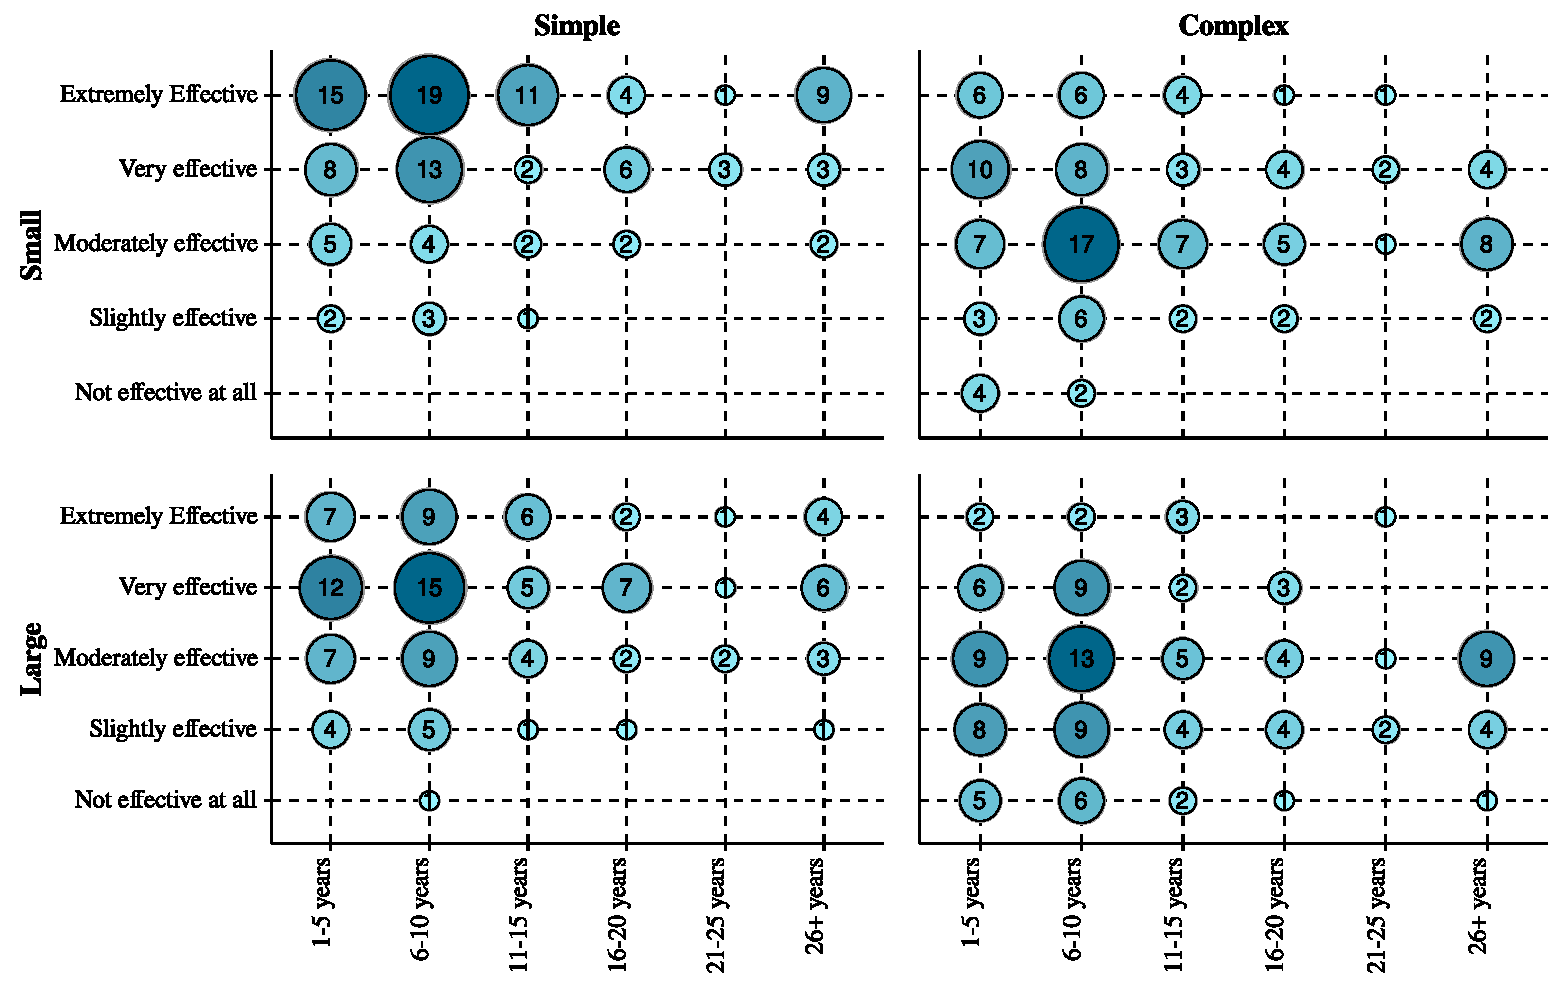
\includegraphics[width=\textwidth]{ConflictComplexityVsSize.pdf}
\caption{Effectiveness of developer tools in supporting varying levels of size and complexity (by developer experience). Values are number of responses per answer, and bubble size indicates the number of responses for comparison purposes.}
\label{size_vs_complexity}
\end{figure*}

\underline{\textit{History Exploration:}}
Notably, many tool-related complaints in the interviews came from within the context of the \textit{Archeology Lens}~\cite{mihai_lenses}, meaning that developers find tool support lacking when trying to explore older history to understand the evolution of a project or even a single line of code. In the words of P1, 

\begin{displayquote}
\textit{``Give me a way to explore the history. To drill down, to go back up, you know? To resurface and understand what happened.''}
\end{displayquote}

The reality for developers using Git for more advanced history exploration use cases is that tool support is thin. P1, as someone who frequently dives deep into Git history, had resorted to writing his own scripts to better find the parts of the history that he really cares about. P9 described a similar tool developed by their open-source project which fills the need for more advanced branch diffing:
\begin{displayquote}
\textit{``git-diff will just do the diff based on the SHAs... we're adding metadata and cherry picking, [so] the SHAs are always going to be changing... this actually allows us to do a comparison based on SHA but then fall back to author and commit title and metadata information... It also hooks into GitHub labels and uses the labels on the project to do some more advanced heuristics.''}
\end{displayquote}

P9 says that all of these changes are in an attempt to create something that will \textit{``essentially create a true diff''.}
This suggests that current tools have not been able to keep up with the rapid expansion of metadata that Git and Github are able to provide, to the extent that projects will divert resources to create a tool for more advanced diffing functionality. 

\begin{table}[!]
\renewcommand{\arraystretch}{1.3}
\caption{Survey Participant Toolset (Top 10 tools)}
\label{survey_toolset}
\centering
\begin{tabularx}{0.45\textwidth}{@{}r|*{10}{C}c@{}c@{}}
\toprule
Tool & \# Participants & Description\\
\midrule
Git	& 37 & Version Control System\\
Vim/vi & 17 & Text Editor\\
Text Editor (unspecified) & 14 & Text Editor\\
Git Diff & 11 & Diffing Tool\\
GitHub & 11 & Website\\
Eclipse & 10 & IDE\\
KDiff3 & 9 & Diff \& Merge\\
Meld & 8 & Diff \& Merge\\
SourceTree & 8 & Git/Hg Desktop Client\\
Sublime Text & 7 & Text Editor\\
\bottomrule
\end{tabularx}
\end{table}
\section{Implications}\label{implications}
This paper examines the ways that software practitioners perceive the merge conflict resolution process.
We discuss the implications, from their perspective, and break down the implications for researchers, tool builders, and managers.

\subsection{For Researchers}
Our results inform future research in the area of merge conflicts from a human perspective.
Our findings from Sections~\ref{artifact-based-factors} and \ref{knowledge-based-factors} indicate that practitioners' knowledge gaps during merge conflict resolution are of similar importance as code-centric metrics of code complexity and SLOC.

\textit{Complexity of conflicting lines of code} (F1) and \textit{Your knowledge/expertise in the area of conflicting code} (F2) represent our top two factors in the assessment of difficulty when approaching a merge conflict.
These factors illustrate the divide between common metrics and the information needs of practitioners performing the resolution.
 
Our findings confirm that informativeness of commit messages (N8) has a moderate impact on practitioners' perceptions, but with seven other factors ranked higher, it receives more research focus than might otherwise be warranted.
Future research should also focus on knowledge- and comprehension-based difficulties of  merge conflict resolutions.

We also highlight nine unmet needs and nine factors of difficulties which have no statistical differences across experience, project size, open/closed source, or role.
This population-wide consensus indicates that practitioners unanimously want these unmet needs resolved, and these factors lessened.

\subsection{For Tool Builders}
Tools are meant to solve problems, but our results show that addressing the human needs of  practitioners in the areas of context-awareness and information retrieval during merge conflict resolutions is also important.
Mainstream tools must help find expertise in areas of conflicting code.
This result agrees with and adds to work done by Costa et al.~\cite{CostaSarma}.
Additionally, tool builders need to provide more ways for practitioners to gather information about the change impact of merge conflicts, including rationales for those changes when possible.

Version control systems provide a easy way of storing and retrieving recent history, but examining older version history at scale is still an open concern among practitioners.
Tool builders should work to address this unmet need by leveraging research into search systems for developer-assistance~\cite{nabi2016putting} and machine learning-based code assistances~\cite{bradley2011history_exploration} to provide practitioners with more expressive tools for history exploration.

Tools specific to integrators, who merge more often and more frequently than regular practitioners, are lacking in depth of features specific to this group.
Support for more advanced and more specific use cases is critical to supporting those who deal with these large, complex merges. 

\subsection{For Managers}
Practitioners find the merge conflict resolution process to be challenging due to a lack of information, lack of expertise, and a lack of code comprehensibility (N1-N3). 
To reduce these challenges, managers should both encourage and allot time for code reviews and paired conflict resolution sessions. 
Allowing better communication between different stakeholders allows domain experts to express concerns about impacts of changes, allows authors to understand the intentions of others' code changes, and allows practitioners to put the collective knowledge of the group to the task of finding the best resolution for the conflict.

Further work is needed to assist managers with determining the most appropriate pairings of experienced practitioners and newcomers to resolve and prevent merge conflicts.
Expertise recommendation tools such as TIPMerge~\cite{CostaSarma}, Ensemble~\cite{xiang2008ensemble}, or techniques such as the H-Index~\cite{bornmann2005does} should be further examined for applicability in industrial development settings.
\section{Threats to Validity}\label{threats}
\subsubsection{\underline{Construct}}
Interview questions were open-ended and designed to elicit practitioner opinions about the experiences, difficulties, and perceptions of merge conflicts.
The particular factors and needs were determined after concluding all interviews, and thus did not bias interview participants to only factors previously mentioned.
Survey questions were created using factors found through card-based unitization.
This methodology allowed us to capture the common themes that practitioners experience when working with merge conflicts, but might have allowed themes specific to particular sub-groups to be unrepresented in our results.
\subsubsection{\underline{Internal Validity}}
Central tendency bias~\cite{guilford1954psychometric} is an issue in studies with 5-point Likert scales, since participants tend to choose less opinionated answers.
We lessen this effect by examining the answers in comparison to each other, as opposed to analysis of absolute mean values.
Because we use this method to highlight stronger answers by degree, this also means that we may have missed subtle trends across our data that may have been visible otherwise.

\subsubsection{\underline{External Validity}}
Interview results may not be generalizable to all practitioners due to a small sample size.
In order to reduce this effect, interview participants were selected from open- and closed-source projects, varying industries, and varying project sizes (see Table \ref{interview_demographics}).
To expand and confirm our interview results, we used a survey of 162 practitioners to ensure our results match with trends in the larger software development community.
We also recognize that recruitment of participants through digital communication methods is subject to self-selection bias and non-response bias.

\subsubsection{\underline{Reliability}}
The possibility exists that practitioner opinion will change over time or with a different sample group of survey participants.
By surveying 162 practitioners from varying roles, experience levels, and team sizes, we take a representative sample of the larger population of software practitioners.
Population sampling, including surveys, are traditionally validated for reliability through disclosure of response rates.
However, we used social media and mailing lists which do not allow accurate measurements of the number of individuals that read our recruitment requests.
Therefore we do not report a survey response rate.

The interview script and survey questions can be found on our website, see~\cite{companion_site}.


\section{Related Work}\label{related_work}
\section{Conclusion}\label{conclusion}
Merge conflicts interrupt 
Our work explores the human perceptions of merge conflict resolution in version control systems. We conducted an analysis of 10 interviews and confirmed our findings with a survey of 226 developers.

We asked how developers approach merge conflicts and found that they identify 8 factors of importance for the initial evaluation of merge conflict difficulty. 
We then asked which factors impact the difficulty of a merge conflict resolution and found 10 factors that impact the difficulty of the merge conflict resolution process. 
These sets of factors serve as a way to inform managers and future research about merge-conflict-related difficulties of software developers.

We also asked if developer tools meet their needs for merge conflict resolutions and found 6 improvements which developers would like to see in these tools. In addition, we share specific tool needs from our interviews to give an idea of what people really struggle with in their merge conflict resolution workflows.

Essentially, this paper contributes an empirical study that can act as a basis for reasoning and further investigation about merge conflicts' perceived difficulties and the support that developers are getting from tool builders. 
%\input{miscellaneous} %% DELETE THIS SECTION BEFORE PUBLISHING
\section*{Acknowledgments}

We thank Iftekhar Ahmed, Amin Alipour, Alex Hoffer, Michael Hilton, Sruti Ragavan, and the anonymous reviewers for their valuable comments on earlier versions of this paper.
We also thank all of our interview and survey participants, especially those who helped distribute survey links.
This research was partially supported by NSF grants IIS-1559657, CCF-1253786, and ...[Danny's grants].


\bibliographystyle{IEEEtran}
\bibliography{Bibliography}{}

\end{document}


